% Chapter Template
\chapter{State of the art techniques}

\label{Chapter2} % Change X to a consecutive number; for referencing this chapter elsewhere, use \ref{ChapterX}

\lhead{Chapter 2. \emph{State of the art techniques}} % Change X to a consecutive number; this is for the header on each page - perhaps a shortened title
 Research in any field is a continuous process. It is meaningless to propose altogether new approaches ruling out the techniques proposed in the literature. Hence a careful study of the state-of-the-art techniques is necessary. It will give a clarity of the approaches that could be incorporated, improved or improvised in the research study of interest. The experimental platform that is being aimed in this thesis is largely an integration of various available techniques which makes literature review even more crucial. This chapter discusses the various methods and techniques proposed in the literature for addressing the problems described in Section~\ref{sec:problem_statement}.
\section{Human behavior understanding} % Main chapter title
The human behavior understanding could be approached from non-verbal and verbal communication perspective. The non-verbal communication is rich in information. It conveys to the receiver the emotion, the attitude, the deeds and even the health of the human. Vision based motion capture and analysis has been studied widely and a condensed summary of the approaches developed during the past three decades are presented in surveys \cite{Moeslund2001231}\cite{Moeslund200690}\cite{Poppe20074}. These surveys have investigated vision based human motion capture and analysis in general, however our particular focus is to use RGB-D sensors to this purpose. Human pose estimation has traditionally suffered from two main problems
\begin{itemize}[leftmargin={1cm},topsep={0pt},itemsep={0pt},partopsep={0pt},parsep={0pt}] 
\item Necessary to adopt an initialization pose.
\item Losing track after a few frames.
\end{itemize}
Alternative techniques which do not require to adopt an initialization pose and estimate pose from single depth images are proposed by Shotton et al., \cite{shotton2013real} \cite{shotton2013efficient}. The studies propose two approaches shown in Fig.~\ref{fig:kinect_pose} namely \emph{Body Part Classification (BPC)} and \emph{Offset Joint Regression (OJR)} for human pose estimation which are capable of accurately predicting the 3D positions of body joints using single depth images without using any temporal information. By using simple depth pixel comparison features, and parallelizable decision forests \cite{breiman2001random}, both approaches could run in realtime on consumer hardware even without tracking a full body model. This is crucial in HRI because there are scenarios in which the human might be sitting and there will be lot of occlusions. 
\begin{figure}
\centering
\begin{subfigure}[t]{0.48\textwidth}
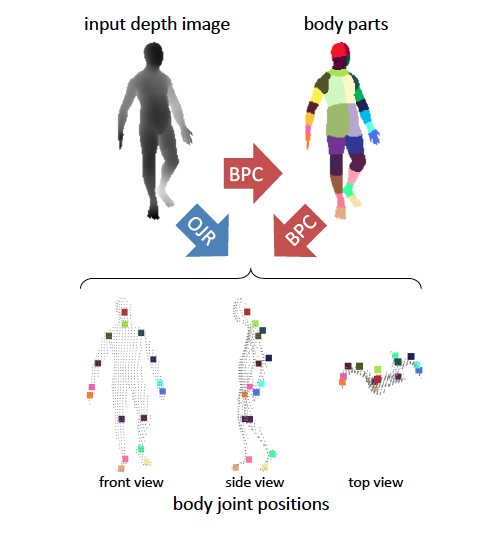
\includegraphics[width=\textwidth]{assets/kinect_approaches.png}
\caption[Human pose estimation]{Human pose estimation \cite{shotton2013efficient}}
\label{fig:kinect_pose}
\end{subfigure}
\begin{subfigure}[t]{0.48\textwidth}
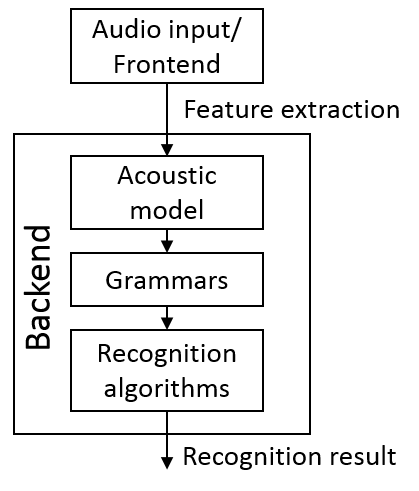
\includegraphics[width=\textwidth]{assets/speech_recognition.png}
\caption[Speech recognition flow]{Speech recognition flow}
\label{fig:speech_recog}
\end{subfigure}
\caption[Human behavior understanding]{Human behavior understanding}
\label{fig:behavior_understand}
\end{figure} 
Unlike the approaches used in the Kinect SDK, the approach presented in \cite{buys2014adaptable} uses both the depth and color (RGB-D) data for human body detection and pose estimation using a customizable human kinematic model. This method makes use of iterative refinement technique in order to estimate the pose of multiple people among clutter and occlusion. Moreover this approach requires less training data and the algorithm is open sourced as part of PCL library \cite{rusu20113d}.  

In the publication by Microsoft research \cite{han2013enhanced}, a background study on various algortihms used for non-verbal human activity analysis is presented. Recently \cite{KinectSDK2014} data-driven machine learning approaches like neural networks, Support vector machines, clustering, decision trees and bayesian networks are being exploited to this purpose. In \cite{KinectSDK2014}, an AdaBoost (Adaptive Boosting) algorithm \cite{freund1997decision} which is one of the top 10 data mining algorithms, is used to efficiently detect the gestures. This approach has been proved to be robust with accuracy as high as 94.9\%. 

The verbal communication has been widely used in human computer interaction systems since many years. Thanks to the integration of Automatic Speech Recogntion (ASR) in the computing devices, there exists a wide variety of algorithms like Hidden markov model, Dynamic time warping etc., in literature \cite{reddy1976speech} \cite{lippmann1997speech} and software toolkits \cite{SpeechSdk} that implement these algorithms. The schematic representation of speech recognition workflow is shown in Fig.~\ref{fig:speech_recog}. The front end receives the audio input, processes it and perform feature extraction. Then a language dependent acoustic model that represents the relationship between audio signal and linguistic units is used to extract language specific features. The recognition rules described in grammar files \cite{Hunt:04:SRG} will then be used to recognize speech by the chosen algorithm.

\section{Localization of humanoid robot} % Main chapter title
The localization of humanoid robots is a challenging issue, due to rough odometry estimation, noisy onboard sensing, and the swaying motion caused by walking \cite{cervera2012localization}. For most of the humanoid robots the reference frame will be fixed to the torso as is the case for the Nao. So the basic idea is to track the torso of the Nao or any other position with the known transformation from the torso.
\subparagraph{Artificial marker based approaches}
Tracking rectangular fiducial markers can be interesting if one could embed those markers on the humanoid robot. This is one of the simplest and cheapest solution in terms of the computational power as it uses simple image processing algorithms. ARToolKit \cite{kato1999marker} implements video tracking libraries which can calculate the real camera position and orientation relative to physical markers in real time. Marker detection frameworks perform simple edge detection techniques to identify markers of known geometry from incoming images of a calibrated camera. The workflow is shown in Fig.~\ref{fig:artoolkit}
\begin{figure}[H]
\centering
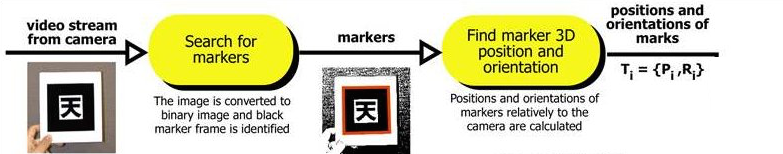
\includegraphics[width=0.8\textwidth]{assets/artoolkit.eps}
\caption[Marker tracking using ARToolKit]{Marker tracking using ARToolKit. {Adapted from \cite{kato1999marker}}}
\label{fig:artoolkit}
\end{figure}
\subparagraph{Point cloud based approaches}
\label{ssec:pcl}
The Point Cloud Library (PCL) \cite{rusu20113d} which is one of the most widely used 3D perception software library, has collection of state-of-the-art algorithms and tools to process 3-D data. Point cloud library provides an excellent infrastructure for the object recognition and 6-DOF pose estimation pipeline by offering a wide variety of robust local and global features \cite{aldoma2012point}. 

The computation of pose of an object of known geometry requires the point cloud of the mesh of the object to begin with. The 3D features known as descriptors of the model are computed and stored to be used during the recognition phase.  During the recognition, at first descriptors (local or global) of the incoming point cloud from sensor are computed followed by segmentation and correspondence matching is performed with all the known models in the database. This is followed by an correspondence grouping using Random Sampling Consensus (RANSAC) to remove the outliers. Following this, a least square optimization is performed to obtain the rotation and the translation from exact point correspondences. Apart from the object recognition and pose estimation pipeline, PCL provides a comprehensive algorithmic base for the tracking of 3D objects using Monte Carlo sampling techniques \cite{RUeda2012}. PCL also has non-probabilistic tracking algorithms like Pyramidal Kanade Lucas Tomasi (KLT) Tracker in its tracking module.
\subparagraph{Probabilistic approaches}
\label{ssec:prob_approaches}
Probabilistic localization algorithms are variants of the Bayes filter \cite{thrun2005probabilistic}. The pose of the robot is represented in a probabilistic manner called the \emph{belief} which is a posterior distribution over the state space. The Bayes filter \cite{thrun2005probabilistic} forms the basis of Markov localization algorithms. Extended Kalman Filter (EKF) based localization is one of the initial developments to be used in non-linear state models (since robot motion model is non-linear). However they suffered problems of uni-modal distribution (gaussian) assumption and failing to solve global localization problem. The particle filter \cite{thrun2005probabilistic} which is an alternative non-parametric implementation of bayes filter, represents the posterior by a set of samples drawn from the distribution. Such a representation is approximate, but it is nonparametric, and therefore can represent a much broader space of distributions. Monte-carlo localization (MCL) \cite{fox1999monte} is a version of Markov localization that uses fast sampling techniques to represent the belief and it introduces probabilistic motion and perceptual models into the particle filter framework.
	
Studies on robot localization, obstacle mapping, and path planning in multilevel 3D environments by equipping Nao with a consumer-level depth camera have been reported in \cite{maier2012real}. This study provides real-time solution while maintaining a 3D environment representation and estimating the 6D pose of the robot. Given the estimated 6D pose of the humanoid and a sequence of depth images, this approach continuously builds a local 3D representation of the current state of the environment containing also non-static obstacles. This learned 3D representation is then used for real-time planning of collision-free paths. 
	
While \cite{maier2012real} presented an approach wherein a depth camera is fixed to the humanoid robot, in \cite{cervera2012localization} localization and motion planning in smart home environment have been proposed using an external depth camera, which is very close to the scenario of this thesis. The MCL technique is used for the pose estimation of the torso of the humanoid robot and this information is used for the closed loop navigation control.
	
In \cite{choi2013rgb} a robust particle filter parallelized on a GPU that can track a known 3D object model over a sequence of RGB-D images is proposed. Unlike PCL object tracking algorithm \cite{rusu20113d} which maintains only one reference point cloud, this approach uses multiple viewports rendered in GPU with different poses and each particle searches the closest rendering from the viewports and likelihood evaluation is performed by transforming the closest rendered result with the current particle state. This approach has been proved to be faster and also accurate than the PCL tracking. However the implementation of this algorithm is not open.
\section{Behavioral frameworks} % Main chapter title
The users of social robots do not have necessary backgrounds in robotics, computer programming or design of robot behaviors. This lead to the development of several visual programming languages which allow non-programmers to create robot applications. Most of the available visual programming softwares allows to choose among many prebuilt behavioral blocks and connecting them to one another to get the desired flow of action \cite{MSRS4} \cite{Choregraphe}. These programs are very intuitive and allow the users to realize complex sequence of movements and sequential behaviors. But programming dynamic behaviors still remains challenging. This is primarily due to fact that the users have to think about the data flow between various blocks by appropriate connections between them. When it comes to designing complex dynamic behaviors this task becomes very tedious and time consuming. There are many solutions proposed in the literature that address the dynamic control problem. For instance Gostai's Universal Robotic Body Interface(URBI) \cite{baillie2008urbi} and Task description language (TDL) \cite{simmons1998task} are programming languages developed specifically for robot programming. URBI provides a modern object-oriented scripting language that allows the organization of code into different processes that either run sequentially or in parallel, and it also provides tools for process execution monitoring. In TDL which was developed as a C++ extension, the code is organized into task trees, which encode the hierarchical decomposition of tasks as well as the synchronization of constraints between tasks. More recently, specialized operating systems have been proposed, such as ROS \cite{quigley2009ros}, which organize code into distributed asynchronous modules that exchange data using a data subscription protocol. These solutions manage the integration and communication between different types of hardware and software and support the implementation of reaction, as well as behavioral specification. However, these programs have been produced by robot developers and are targeted at this community, which means that they are not intended to be used by non-roboticists and a solid background in computer science/robotics is required for their use.

A non-domain-specific solution called \emph{Targets-Drives-Means (TDM)} is proposed in \cite{berenz2014targets} taking into account the aforementioned needs. TDM proposes a programming paradigm where temporal independent dynamic behaviors blocks run in parallel. The logic of the program is not expressed using communication links in a flowchart, but by the use of specialized dynamic components that regulate the activation status and the priorities of the behaviors. However there does not exist an intuitive interface for the behavior design yet and this framework is not open.
\section{HRI design and evaluation} % Main chapter title
For the systems involving humans, it is essential to understand how the user feels about the system and HRI is no exception. A successful human study in HRI requires careful planning and design. In \cite{bethel2010review}, a set of questions when planning and designing a human study in HRI is presented. In addition to this \cite{bethel2010review} also gives a list of recommendations for the experimental design and study execution. Data collection is one of the important steps in the evaluation process. In \cite{Rogers2011} an insight of the design process of an interactive system is presented. It discusses five key issues in the data gathering such as identifying participants, relationship with participants, setting goals, triangulation and importance of conducting pilot studies. An extensive review of HRI evaluation methods presented in \cite{bethel2010review} summarises five primary methods such as \emph{Self assessments}, \emph{Interviews}, \emph{Behavioral measures}, \emph{Psychophysiology measures} and \emph{Task performance metrics}. Each of these methods has advantages and disadvantages. However the study claims that it is possible to overcome these disadvantages by using three or more appropriate methods of evaluation. An effort to identify a set of common metrics to be used in task-oriented HRI can be found in \cite{Steinfeld2006}. This study proposes a set of metrics to evaluate the user, robot and the team (human-robot) performances. Bartneck et al., \cite{bartneck2009measurement} emphasize the need for standardized measurement tools for human robot interaction. This work presents measurements tools in the form of questionnaires for five key concepts in HRI: anthropomorphism, animacy, likeability, perceived intelligence, and perceived safety. All the evaluation techniques rely on the statistical tools for validating the results and generalizing the phenomena. A summary of commonly used statistical tools for the data analysis in HRI is summarized in Appendix~\ref{AppendixA}.

\section{Summary}
In this chapter a review of the literature which are most relevant to this thesis research is presented. The literature review helped to identify the appropriate techniques that could be used in the development of experimental platform. The key decisions made are shown in the Table~\ref{table:review_decisions}

\begin{table}[H]
\centering
\small
\caption{Identified techniques from state-of-the-art}
\label{table:review_decisions}
\begin{tabular}{ | l | p{10cm} |}
\hline
  \textbf{Problem to be addressed} & \textbf{Identified solution}
  \tabularnewline \hline
  
  Human behavior understanding & The Kinect SDK \cite{KinectSDK2014} will suffice the human skeleton tracking. The Visual gesture builder tool that is shipped with Kinect SDK could be used for gesture creation and recogntion. As far the speech recognition is concerned Microsoft Speech Platform 11 \cite{SpeechSdk} will be used.
                                          \tabularnewline\hline
                                          
  Localization of humanoid robot & The artificial marker based approaches seems to be the cheapest solution since we will be sharing the same sensor for motion recogntion as well. The ALVAR marker tracking library \cite{ALVAR} will be used to this purpose. 
                                          \tabularnewline\hline
  
  Application infrastructure & It has been decided to develop a \textbf{\emph{proprietary application infrastructure}} as existing solutions like ROS \cite{quigley2009ros} is not cross-platform and the Kinect sensor drivers for Linux are not mature enough at the time of this writing.
                                          \tabularnewline\hline

  Behavior framework & It has also been decided to develop a \textbf{\emph{new behavior design and execution framework}} as the existing solutions are not complete and they do not offer an end-to-end solution for naive users wanting to design HRI scenarios.
                                          \tabularnewline\hline

  HRI evaluation & The \emph{Self-assessment} \cite{bethel2010review} techniques will be adopted and data collection will be done on a set of identified participants. Statistical analysis will be performed on the collected data to measure usability metrics like \emph{effectiveness}, \emph{efficiency} and \emph{satisfaction}
                                          \tabularnewline\hline
\end{tabular}
\end{table}